\begin{titlepage}

%\center{\fontsize{4cm}{5cm}\selectfont VOTCA-CT}
%\center{\fontsize{1.5cm}{3cm}\selectfont USER MANUAL}

\center{\huge \sc Charge Transport Simulations}
\vspace*{1cm}
\center{\Large \sc User Manual}

\vspace*{3cm}
\center{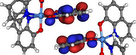
\includegraphics[width=0.6\columnwidth]{fig/logo}}
\vspace*{1cm}

%\center{\footnotesize{compiled from: \hgid}}
%\center{\footnotesize{Programs version: \refhgid}}
%\vspace*{1cm}
%\center{
%\large{\copyright \hspace*{0.1cm} VOTCA development team}
%}
%\vspace*{0.5cm}
\vfill
\center{\large{\today}} \\
% %\vspace*{-0.3cm}
\htmladdnormallink{\color{black}\large{www.votca.org}}{http://www.votca.org}
\end{titlepage}

\section*{Disclamer}
This manual is not complete. The best way to start using the software is to look at provided tutorials. The reference section is generated automatically from the source code, so please make sure that your software and manual versions match.  

\section*{Citations}
Development of this software depends on academic research grants. If you are using the package, please cite the  following papers \\

\vspace{0.1cm}
\noindent
~\cite{ruehle_microscopic_2011} V. R\"uhle, A. Lukyanov, F. May, M. Schrader, T. Vehoff, J. Kirkpatrick, B. Baumeier, D. Andrienko,
``Microscopic simulations of charge transport in disordered organic semiconductors'', \htmladdnormallink{\color{black} {\itshape J. Chem. Theor. Comp.} 2011}{http://dx.doi.org/} \\

\vspace{0.1cm}
\noindent
~\cite{ruehle_versatile_2009} V. R\"uhle, C. Junghans, A. Lukyanov, K. Kremer, D. Andrienko, 
``Versatile Object-oriented Toolkit for Coarse-graining Applications'',
\htmladdnormallink{ \color{black} {\itshape J. Chem. Theor. Comp.} 5, 3211, 2009}
{http://dx.doi.org/10.1021/ct900369w}

\section*{Development}
The core development is currently taking place at the Max Planck Institute for Polymer Research, Mainz, Germany.

\section*{Copyright}
\votcact is free software. The entire package is available under the Apache License. For details, check
the LICENSE file in the source code. The \votcact source code is available on our homepage, \htmladdnormallink{\color{black}\large{www.votca.org}}{http://www.votca.org}.

\vfill